%%Intro to the Literature Review
    

In this chapter we will provide a more comprehensive analysis of the existing research surrounding ladder lotteries. Let {\sc x} be 
a ladder lottery or permutation. 
Throughout this thesis a number of algorithms are presented. Many of these algorithms use the following auxiliary functions: 
\begin{enumerate}
    \item {\sc Print(x)}: Prints {\sc x}.
    \item {\sc Swap(x,y)}: Swaps {\sc x, y}.
    \item {\sc Sort(x)}: Sorts {\sc x} in ascending order.
    \item {\sc Sorted(x)}: Returns true if {\sc x} is sorted in ascending order, else returns false.
    \item {\sc Max(x)}: Returns the maximum element in {\sc x}.
    \item {\sc Min(x)}: Returns the minimum element in {\sc x}.
\end{enumerate}

The study of ladder lotteries as mathematical objects began in 2010, in the paper
Efficient Enumeration of Ladder Lotteries and its Application, written by Matsui, Nakada, Nakano Uehara and Yamanaka~\cite{A1}. 
In this paper the authors present the first algorithm for generating $OptL\{\pi\}$ for some  
arbitrary permutation $\pi$. Since this paper emerged, there have been 
a number of other papers written about ladder lotteries.
These papers include The Ladder Lottery Realization Problem,
Optimal Reconfiguration of Optimal Ladder Lotteries, 
Efficient Enumeration of all Ladder Lotteries with K Bars,
Coding Ladder Lotteries and
Enumeration, Counting, and Random Generation of Ladder Lotteries.
This thesis is also heavily influenced by Efficient Enumeration of Ladder Lotteries and its Application. Throughout Chapter 2, 
we elaborate on the aforementioned papers pertaining to ladder lotteries.


%$input review of first paper
\section{Efficient Enumeration of Laddder Lotteries and its Application}

%%Intro
\subsection{Introduction}
In their paper, \textbf{Efficient Enumeration of Ladder Lotteries and its Application},
the authors provide an algorithm for generating $OptL\{\pi\}$ 
for any $\pi$, in $\mathcal{O}(1)$ per ladder \cite{A1}. This is the first algorithm for generating $OptL\{\pi\}$. 
To see this algorithm please refer to 
Alg.\ref{Alg:FindAllChildren}. The paper also presents the number 
of ladder lotteries in $OptL\{(11, 10, 9, 8, 7, 6, 5, 4, 3, 2, 1)\}$ which is 
$5,449,192,389,984$ \cite{A1}.There are also four other algorithms in 
this section, none of which are found in the paper \emph{Efficient Enumeration of Ladder Lotteries and its Applications}. The 
algorithms are Alg.\ref{Alg:RootLadder}, Alg.\ref{Alg:RightSwap}, Alg.\ref{Alg:LeftSwap} and Alg.\ref{Alg:ShiftChildren}.
These algorithms are used to perform mandatory steps in \ref{Alg:FindAllChildren}. These algorithms are novel.\par 
The authors' algorithm is known as \emph{FindAllChildren}. It is based on several key concepts, the most 
important of which is the \emph{local swap operation}. This is the 
minimal change operation that transitions from one ladder in $OptL\{\pi\}$ to the 
next ladder. The local swap operation is essentially a 180 degree rotation
of three bars in the ladder, such that the bottom
bar is rotated to the top, the middle bar stays in the middle and the top bar
is rotated to the bottom. If the bars undergo a 180 degree rotation to the right, 
then this is known as a \emph{right swap operation} and 
if the bars udergo a 180 degree rotation to the left then this 
is known as a \emph{left swap operation} \cite{A1}. To go to the next ladder in the set, 
the current ladder, $l_{i}$, udergoes a right swap operation 
to get to ladder $l_{i+1}$. See Fig.\ref{fig:rightSwap} for an exmaple of a 
local swap operation. The \emph{route} of an element is the sequence of bars in the ladder that an element must cross 
in order to reach its correct position in 
the identity permutation \cite{A1}. The sequence is ordered from top left to bottom right.
Note, that each bar has two elements that cross it, 
therefore the bar belongs to the route of the greater of the two elements. 
It is important to note that when a right swap operation occurs, 
two of the three bars belong to the route of a unique greater element and one bar belongs
to the route of a unique lesser element. Once rotated, the bar of the lesser element is 
moved above the bars of the greater element.\par
The \emph{clean level} refers to the smallest element 
in $\pi$ such that none of its bars have undergone a right swap operation \cite{A1}.
If there is no such element, then the clean level is the maximum element in $\pi$ + 1.
The \emph{root ladder} is the only ladder in  the set with a clean level of 1; in 
other words, the root ladder is the only ladder in which no bars have undergone 
a right swap operation. The root ladder is unique to $OptL\{\pi\}$. To see the root ladder 
of $OptL\{(4,5,6,3,1,2)\}$ please refer to figure Fig.\ref{fig:root}. The root ladder is
also the \emph{first ancestor  ladder} in $OptL\{\pi\}$. Insofar as the enumeration algorithm 
is based on performing a right swap operation on a pervious ladder, then every other 
ladder in $OptL\{\pi\}$ must have at least one right swap operation. Since the root ladder has
no right swap operations, then it must be an ancestor of every other ladder.\par

%%Root ladder subsection
\subsection{The Root Ladder in Detail}
The authors provide a good description of the root ladder, however they do not provide an algorithm 
for creating the root ladder. Since the root ladder is an ancestor to every other ladder in $OptL\{\pi\}$, 
the root ladder cannot be created using the same algorithm as every other ladder. This thesis provides such 
an algorithm in Alg.\ref{Alg:RootLadder}.\par

\begin{algorithm}
	%%\setstretch{1.35}
	 %% \algsetup{linenosize=\tiny}
	\begin{algorithmic}[1]
		\Function {CreateRoot}{$ladder[2(N-1)-1][N-1]$, $\pi$, $N$, $row \gets 1$}
			\If{$N=1$}
				\State return
			\EndIf
			\State $largestIndex \gets$ index of largest element in $\pi$
			\For{$i \gets largestIndex+1$, $i \leq N$, $i \gets i+1$}
				\If{$\pi_{largestIndex}>\pi_{i}$ $AND$ $largestIndex < i$}
					\State $column \gets i$
					\If{This is the first bar to be added}
						\While{bar cannot be added}
							\State $row \gets row+1$
						\EndWhile
						\State $ladder[row][column] \gets 1$
					\Else 
						\State $row \gets row+1$
						\State $ladder[row][column] \gets 1$
					\EndIf
				\EndIf
			\EndFor
			\State $\pi \gets \pi - largestElement$
			\State $CreateRoot(ladder, \pi, N-1, row \gets 1)$
		\EndFunction

	\end{algorithmic}
	\caption{The algorithm for creating the root ladder of $OptL\{\pi\}$}
	\label{Alg:RootLadder}
\end{algorithm}\pagebreak



Let $ladder$ be a two dimensional array, let $\pi$ be the current state of the permutation, let $N$ be the 
size of $\pi$, let $row$ be the current row in the ladder. First, the index of the largest element in $\pi$ is assigned to $largestIndex$. 
Once found, the algorithm loops from $largestIndex+1$ to $N$. If $\pi_{largestIndex}>\pi_{i}$ then a bar is to be added to 
$ladder$ at $row,column=i$. There are two cases for calculating the $row$. 
\case{\emph{First bar is being added}}{This is the first bar to be added to the route of the largest element. 
$row$ is incremented until a bar can be added to $ladder$ at $row$ 
and $column$. A bar can be added if neither of its endpoints are touching the endpoints of any other bar.}
\case{\emph{Second or greater bar is being added}}{If this is second or greater bar to be added to the route of the 
largest element in $\pi$ then $row \gets row+1$.}
Once all the bars for the route of the largest element have been added, the largest element from $\pi$ is removed, 
$N \gets N-1$ and $row \gets 1$. Then the algorithm makes a recursive call.

\begin{lemma}
	The time complexity for $CreateRoot$ is $O(N^{3})$
\end{lemma}
\begin{proof}
	The outer for-loop of the function runs from some arbitrary index to $N$ on each function call. The inner for loop runs at most 
	$2(N-1)-1$ times which is reduced to $N$. Thus, we get $O(N^{2})$. The following 
	recursion holds, $CreateRoot(N-K) = CreateRoot(N-K+1) + O((N-K)^{2})=CreateRoot(N-K+2) + O((N-K)^{2}) + O((N-K+1)^{2})\dots $. Which is 
	reduced to $O(N(N+1)(2N+1)/6) = O(N^3)$. QED.
\end{proof}
\pagebreak


\begin{figure}[!htp]
	\begin{minipage}{0.4\textwidth}
		\begin{center}

			%%drawing the lines
			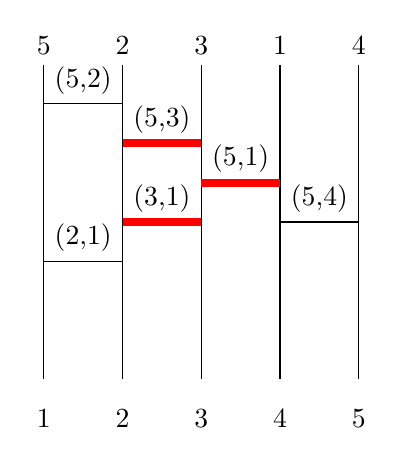
\begin{tikzpicture}
				\draw(0, 0) to (0, 4) node[above]{5};
				\node at (0, -0.5){1};

				\draw(1, 0) to (1, 4) node[above]{2};
				\node at (1, -0.5){2};


				\draw(2, 0) to (2, 4) node[above]{3};
				\node at (2, -0.5){3};

				\draw(3, 0) to (3, 4) node[above]{1};
				\node at (3, -0.5){4};


				\draw(4, 0) to (4, 4) node[above]{4};
				\node at (4, -0.5){5};

				%%drawing the bars

				%%5's route
				\draw(0, 3.5)to (1, 3.5);
					\draw node at (0.5, 3.8) {(5,2)};
				\draw[line width=1mm, red](1, 3) to (2, 3);
					\draw node at (1.5, 3.3) {(5,3)};
				\draw[line width=1mm, red](2, 2.5) to (3, 2.5);
					\draw node at (2.5, 2.8) {(5,1)};
				\draw(3, 2) to (4, 2);
					\draw node at (3.5, 2.3) {(5,4)};

				%%4's route, no bars

				%%3s route
				\draw[line width=1mm, red](1, 2) to (2, 2);
					\draw node at (1.5, 2.3) {(3,1)};
				%%2s route
				\draw(0, 1.5) to (1, 1.5);
					\draw node at (0.5, 1.8){(2,1)};
			\end{tikzpicture}
		\end{center}
	\end{minipage}
	\begin{minipage}{0.4\textwidth}
		\begin{flushright}

			%%drawing the lines
			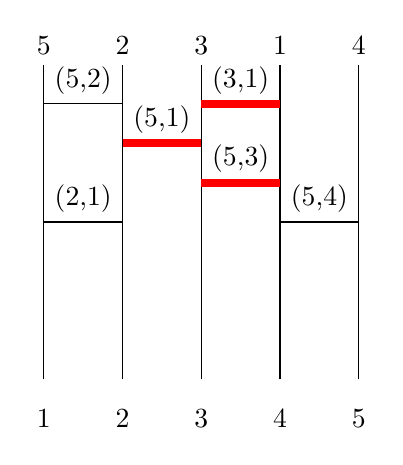
\begin{tikzpicture}
				\draw(0, 0) to (0, 4) node[above]{5};
				\node at (0, -0.5){1};

				\draw(1, 0) to (1, 4) node[above]{2};
				\node at (1, -0.5){2};


				\draw(2, 0) to (2, 4) node[above]{3};
				\node at (2, -0.5){3};

				\draw(3, 0) to (3, 4) node[above]{1};
				\node at (3, -0.5){4};


				\draw(4, 0) to (4, 4) node[above]{4};
				\node at (4, -0.5){5};

				%%Drawing the bars
				\draw(0, 3.5)to (1, 3.5);
					\draw node at (0.5, 3.8){(5,2)};
				\draw[line width=1mm, red](2, 3.5) to (3, 3.5);
					\draw node at (2.5, 3.8) {(3,1)};
				\draw[line width=1mm, red](2, 2.5) to (3, 2.5);
					\draw node at (2.5, 2.8) {(5,3)};
				\draw(3, 2) to (4, 2);
					\draw node at (3.5, 2.3){(5,4)};
				%%4's route, no bars

				%%3s route
				\draw[line width=1mm, red](1, 3) to (2, 3);
					\draw node at (1.5, 3.3) {(5,1)};
				%%2s route
				\draw(0, 2) to (1, 2);
					\draw node at(0.5, 2.3){(2,1)};
			\end{tikzpicture}
		\end{flushright}
	\end{minipage}
	\caption{Example of a local swap operation. When a right swap operation is permformed
	on the left ladder, the result is the right ladder. When a left swap operation is permformed
	on the right ladder, the result is the left ladder.}
	\label{fig:rightSwap}
\end{figure}


\begin{figure}


	\begin{center}
		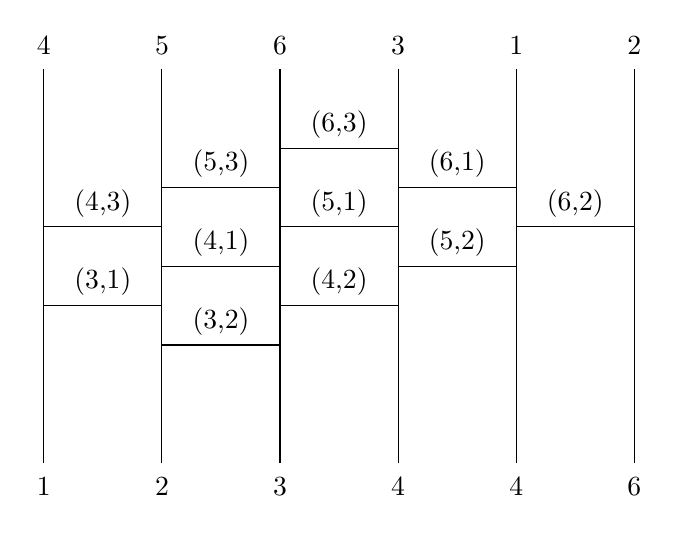
\begin{tikzpicture}
			%%draw the lines
			\draw(0, 0) to (0, 5);
				\node at (0, 5.3){4};
				\node at (0, -0.3){1};

			\draw(1.5, 0) to (1.5, 5);
				\node at (1.5, 5.3){5};
				\node at (1.5, -0.3){2};
			
			\draw(3, 0) to (3, 5);
				\node at (3, 5.3){6};
				\node at (3, -0.3){3};
			\draw(4.5, 0) to (4.5, 5);
				\node at (4.5, 5.3){3};
				\node at (4.5, -0.3){4};
			\draw(6, 0) to (6, 5);
				\node at (6, 5.3){1};
				\node at (6, -0.3){4};
			\draw(7.5, 0) to (7.5, 5);
				\node at (7.5, 5.3){2};
				\node at (7.5, -0.3){6};

			%%draw the bars
			
			%%6's route
			\draw(3, 4) to (4.5, 4);
				\node at (3.75, 4.3){(6,3)};
			\draw(4.5, 3.5) to (6, 3.5);
				\node at (5.25, 3.8){(6,1)};
			\draw(6, 3) to (7.5, 3);
				\node at (6.75, 3.3){(6,2)};
			%%5's route
			\draw(1.5, 3.5) to (3, 3.5);
				\node at (2.25, 3.8){(5,3)};
			\draw(3, 3) to (4.5, 3);
				\node at (3.75, 3.3){(5,1)};
			\draw(4.5, 2.5) to (6, 2.5);
				\node at (5.25, 2.8){(5,2)};
			%draw 4's route
			\draw(0, 3) to (1.5, 3);
				\node at (0.75, 3.3){(4,3)};
			\draw(1.5, 2.5) to (3, 2.5);
				\node at (2.25, 2.8){(4,1)};
			\draw(3, 2) to (4.5, 2);
				\node at (3.75,2.3){(4,2)};

			%%draw 3's route
			\draw(0, 2) to (1.5, 2);
				\node at (0.75, 2.3){(3,1)};
			\draw(1.5, 1.5) to (3, 1.5);
				\node at (2.25, 1.8){(3,2)};
		\end{tikzpicture}

	\end{center}





	\caption{The root ladder for $OptL\{(4,5,6,3,1,2)\}$. Notice how 
	none of the bars have undergone a right swap operation. This is clear 
	when considering that there is no bar of a lesser element above the bar(s)
	of a greater element.} 
	\label{fig:root}

\end{figure}

 %%Save this section for the counting section.
 \begin{theorem}
	 If a ladder from $OptL\{\pi\}$ has not undergone any right swap operations then the ladder is the root ladder. 
	 \label{Theorem:One}
 \end{theorem} 
 \begin{proof}
     The root ladder is defined as the ladder whose clean level is one.
     This means there is no bar of a lesser element above the route a 
     greater element. Keeping in mind that the clean level of the root ladder is one, next consider what is meant by a \emph{child bar}
      which is a bar to the bottom left or right of an arbitrary bar $x$. Within the context of the root ladder, 
      if the left endpoint of the child bar is directly below the right end point of $x$ then the child is a 
     \emph{right child} of $x$. If the right end point of the child bar is directly 
     below the left end point of $x$ then it is a \emph{left child}. Let $x$ belong to the route of element $m$/$Route(m)$.
     If a child is a right child of $x$
	 then it also belongs to the $Route(m)$.
     Let $x$ be a bar representing an inversion with element $m$ and $k$.
     The right child of $x$ is a bar which represents an inversion 
     with $m$ and some element to the right of $k$ termed $k'$. Suppose this was not the case, 
     then this would mean that the right child of $x$ was either a bar representing an inversion 
	 between some element $m'$ such that $m' > m$ or $m' < m$. If $m' > m$ 
	 then this would be a contradiction seeing as $x$ would be above the bar of a route 
     of a greater element which contradicts the definition of the root ladder. On the other hand if 
	 $m' < m$ then $m$ would form an inversion with $m'$ and $x$ would be the bar that uninverted $m$ and $m'$, 
	 but this is also a contradiction seeing as $m' \neq k$ but $x$ uninverts $m$ and $k$. Thus, the right child 
     of $x$ belongs to the same route as $m$ in the root ladder.\par The left child of $x$
     belongs to $Route(l=m-1)$. Suppose this was not the case, 
     then the left child could belong to a route $\geq m$, but if that were the case, this contradicts 
	 the definition of the root ladder seeing as $x$ would be above the route of a greater element. If 
	 $l < m-1$ then the left child of $x$ would be above $Route(m-1)$ which also contradicts the definition 
	 of the root ladder. Therefore, the left child of $x$ must belong to route $l=m-1$. 
	 The second element of the left child of $x$ is $k$. Suppose this was not the case, then 
	 let the second element of the left child be termed $k'$. 
	 $k'$ forms an inversion with $m-1$. But since $m-1 < m$ then $m$ would also form an inversion with $k'$, the 
	 bar corresponding to the inversion $m$ and $k'$ would be $x$. But we already stated that $x$ forms 
	 an inversion between $m$ and $k$, therefore we have another condtradiction. 
	 Therefore, the second element of left child of $x$ must be $k$; the left child of $x$ uninverts elements 
	 $m-1$ and $k$. \par 
	 Please refer to Fig. \ref{Fig:RootChildBars} to view an example of the root ladder for $(3,1,5,2,4)$. Note 
	 that this is a figure of the only ladder in $OptL\{(3,1,5,2,4)\}$.
	 By that the right/left children bars of any given bar 
	 $x$ have not been right swapped, we have proven that if a ladder in $OptL\{\pi\}$ has not undergone 
	 a right swap operation then it must be the root ladder. QED\pagebreak

   
 \end{proof}
 \begin{corollary}
	 If $|OptL\{\pi\}|=1$ then the ladder in $OptL\{pi\}$ must be the root ladder.
 \end{corollary}
 \begin{proof}
	 If there is only one ladder in the set, then that means no bars have been swapped in said ladder. 
	 Thus, it must be the root ladder. QED.
 \end{proof}


 \begin{figure}[!htp]
     \begin{center}
     \begin{tikzpicture}
         \draw(0, 0) to (0, 4);
             \node at(0, 4.3){$3$};
              \draw(0, 3.5) to (2, 3.5);
                 \node at(1, 3.8){$3,1$};
           
             \draw[line width=0.8mm, red](2, 2.5) to (4, 2.5);
                 \node at(3, 2.8){$3,2$};

         \draw(2, 0) to (2, 4);
             \node at(2, 4.3){$1$};
          
         \draw(4, 0) to (4, 4);
              \node at(4, 4.3){5};
                 \draw(4, 3.5) to (6, 3.5);
                     \node at (5, 3.8){$5,2$};
         \draw(6, 0) to (6, 4);
			 \node at(6, 4.3){2};
			 \draw[line width=0.8mm, red](6, 2.5) to (8, 2.5);
			 	\node at(7,2.8){$5,4$};

		\draw(8, 0) to (8, 4);
			\node at(8, 4.3){4};


     \end{tikzpicture}
     \end{center}
     \caption{The root ladder/only ladder in $OptL\{(3,1,5,2,4)\}$ Note that bar 4,2 is the parent of bar 3,2 and 4,1. Also note that 
	 bar 3,2 is the the left child of 4,2 and 4,1 is the right child.}
	 \label{Fig:RootChildBars}
 \end{figure}

%%algorithm
\subsection{$FindAllChildren$}

Let $ladder$ be initilaized as the root ladder. Let $CleanLevel$ be initilaized to $1$. 
Let $N$ be initialized to the max element. The enumeration algorithm 
lists $OptL\{\pi\}$; the authors refer to the algorithm as $FindAllChildren$ \cite{A1}. 
$FindAllChildren$ was used for the bulk of this research, however 
the authors omitted several key steps in the the algorithm. Most notably, they 
omitted the right/left swap operation. Nor do they provide an algorithm 
for permforming a right/left swap operation \cite{A1}. Therefore, I have provided 
the right and left swap operations.
To see $FindAllChildren$ for generating $OptL\{\pi\}$ please refer to Alg.\ref{Alg:FindAllChildren}.
 To see the right/left swap algorithms please 
refer to Alg.\ref{Alg:RightSwap} and Alg.\ref{Alg:LeftSwap} respectively. To 
see an example of a right/left swap operation please refer to Fig.\ref{fig:rightSwap}.
Given an arbitrary bar, $x$, it can be right swapped if and only if there are two bars, $y,z$ where $y \neq z$ 
such that all the following conidtions are met \cite{A1}.
\begin{itemize}
	\item The left end point of $z$ is directly above the left end point of $x$.
	\item The left end point of $y$ is directly above the right end point if $x$.
	\item The right end point of $z$ is directly above the left end point of $y$.
\end{itemize}

Given an arbitrary bar, $x$, it can be left swapped if and only if there are two bars, $y,z$ where $y \neq z$ 
such that the following conditions are met \cite{A1}.
\begin{itemize}
	\item The right end point of $z$ is directly below the right end point of $x$.
	\item The right end point of $y$ is directly below the left end point if $x$.
	\item The left end point of $z$ is directly below the right end point of $y$.
\end{itemize}
In the left ladder in Fig.\ref{fig:rightSwap} bar $x=(3,1)$, bar $y=(5,1)$ and bar $z=(5,3)$. Bar $x$ can be right swapped 
seeing as the three conditions for performing a right swap operation are met.
In the right ladder in Fig.\ref{fig:rightSwap} bar $x=(3,1)$, bar $y=(5,1)$ and bar $z=(5,3)$. Bar $x$ can be left swapped 
seeing as the three conditions for performing a left swap operation are met.


\begin{algorithm}
	\begin{algorithmic}[1]
		\Function{FindAllChildren}{$ladder$, $cleanLevel$, $N$}
			\State $currentRoute \gets N$
			\While{$currentRoute \geq cleanLevel$}
				\State going top left to bottom right 
				\For{$bar \in currentRoute$}
					\State $row \gets$ row of $bar$ in $ladder$ 
					\State $col \gets$ col of $bar$ in $ladder$
					\State $lowerNeighbor \gets ladder[row-1][col]$
					\If{$lowerNeighbor$ is right swappable}
						\State $RightSwap(ladder, bar, lowerNeighbor)$
						\State $FindAllChildren(ladder, y+1, N)$
						\State $leftSwap(ladder, bar, lowerNeighbor)$
					\EndIf
				\EndFor
				\State $currentRoute \gets currentRoute-1$
			\EndWhile
			\State $currentRoute \gets cleanLevel-1$
			\For{$bar \in currentRoute$}
				\State $row \gets$ row of $bar$ in $ladder$ 
				\State $col \gets$ col of $bar$ in $ladder$
				\State $lowerNeighbor \gets ladder[row-1][col]$
				\If{$lowerNeighbor$ is right swappable $AND$ is the rightmost bar of $currentRoute-1$}
					\State $RightSwap(ladder, bar)$
					\State $findAllChildren(ladder, cleanLevel, N)$
					\State $LeftSwap(ladder, bar)$
				\EndIf
			\EndFor
		\EndFunction
	\end{algorithmic}
	\caption{The algorithm for listing $OptL\{\pi\}$.}
	\label{Alg:FindAllChildren}
\end{algorithm}


\begin{algorithm}
	\begin{algorithmic}[1]
		\Function{RightSwap}{$ladder$, $bar$}
			\State $row \gets bar's$ row
			\State $col \gets bar's$ column
			\State $upperNeighbor \gets ladder[row-2][col]$
			\State $rightNeighbor \gets ladder[row-1][col+1]$
			\State $rightSibling \gets ladder[row][col+2]$
			\State $ShiftSubLadder(ladder, rightSibling, 2, 1)$
			\State $Swap(upperNeighbor, ladder[row+1][col+1])$
			\State $Swap(bar, rightNeighbor)$ 
		\EndFunction
	\end{algorithmic}
	\caption{Perform a right swap operation on a bar}
	\label{Alg:RightSwap}
\end{algorithm}
\begin{algorithm}
	\begin{algorithmic}[1]
		\Function{LeftSwap}{$ladder$, $bar$}
			\State $row \gets bar's$ row
			\State $col \gets bar's$ column
			\State $lowerNeighbor \gets ladder[row+2][col]$
			\State $leftNeighbor \gets ladder[row+1][col-1]$
			\State $leftSibling \gets ladder[row][col-2]$
			\State $ShiftSubLadder(ladder, leftSibling, -2, -1)$
			\State $Swap(lowerNeighbor, ladder[row-1][col-1])$
			\State $Swap(bar, leftNeighbor)$
		\EndFunction
	\end{algorithmic}
	\caption{Perform a left swap operation on a bar}
	\label{Alg:LeftSwap}
\end{algorithm}
\begin{algorithm}
	\begin{algorithmic}[1]
		\Function{ShiftSubLadder}{$ladder$, $bar$, $offset$, $index$}
			\If{$ladder[row][col] = 0$}
				\State return
			\EndIf
			\State $row \gets bar's$ row
			\State $col \gets bar's$ column 
			\If{$ladder[row+index][col-index] = 0$ $AND$ $ladder[row+index][col+index] = 0$}
				\State $Swap(ladder[row+offset][col], ladder[row][col])$
			\Else 
				\State $rightChild \gets ladder[row+index][col+index]$
				\State $leftChild \gets ladder[row+index][col-index]$
				\State $ShiftSubLadder(ladder, rightChild, offset, index)$
				\State $ShiftSubLadder(ladder, leftChild, offset, index)$
				\State $Swap(ladder[row+offset][col], Ladder[row][col])$
			\EndIf
		\EndFunction
	\end{algorithmic}
	\caption{Shifts the sub tree of bars up or down the ladder depending on if a right or left swap operation is being performed}
	\label{Alg:ShiftChildren}
\end{algorithm}\pagebreak

The right/left swap functions perform a 180 degree rotation of the bars. When performing a right swap operation, the function 
takes the current bar, $x$, and gets its upper neighbor $z$ and its right neighbor $y$; $x$, $z$ and $y$ meet the 
criteria for performing a right swap operation. The the function calls $ShiftSubLadder$  with the offset value of 
$2$ and the $Index$ value of one. This function ensures that the right sub ladder beginning at the right sibling of $x$, 
located at the same row as $x$ and two columns away from $x$, are shifted down the ladder so that when the right 
swap operation is performed, $z$ will still be above the right sub ladders. To see an example of $RightSwap$ in conjunction with $ShiftSubLadder$ please 
refer to Fig \ref{Fig:SwapAndShift}

\begin{figure}[!htp]
	\begin{minipage}{.4\textwidth}
		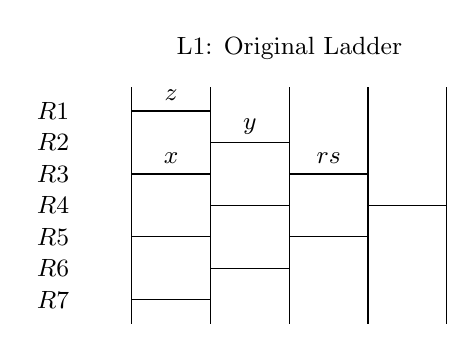
\begin{tikzpicture}
			\node at(2, 3.5){\small{L1: Original Ladder}};
			\draw(0, 0) to (0, 3);
					\node at(.5, 2.9){\small{$z$}};
				\draw(0, 2.7) to (1,2.7);
					\node at(.5, 2.1){\small{$x$}};

				\draw(0,1.9) to (1,1.9);
				\draw(0,1.1) to (1,1.1);
				\draw(0,0.3) to (1,0.3);
			\draw(1, 0) to (1, 3);
				\node at(1.5,2.5){\small{$y$}};
				\draw(1,2.3) to (2,2.3);
				\draw(1,1.5) to (2,1.5);
				\draw(1,0.7) to (2,0.7);
			\draw(2, 0) to (2, 3);
				\node at(2.5, 2.1){\small{$rs$}};
				\draw(2,1.9) to (3,1.9);
				\draw(2,1.1) to (3,1.1);
			\draw(3, 0) to (3, 3);
				\draw(3,1.5) to (4,1.5);
			\draw(4, 0) to (4, 3);

			\node at(-1, 2.7){\small{$R1$}};
			\node at(-1, 2.3){\small{$R2$}};
			\node at(-1, 1.9){\small{$R3$}};
			\node at(-1, 1.5){\small{$R4$}};
			\node at(-1, 1.1){\small{$R5$}};
			\node at(-1, .7){\small{$R6$}};
			\node at(-1, .3){\small{$R7$}};

			
		\end{tikzpicture}
	\end{minipage}
	\begin{minipage}{.4\textwidth}
		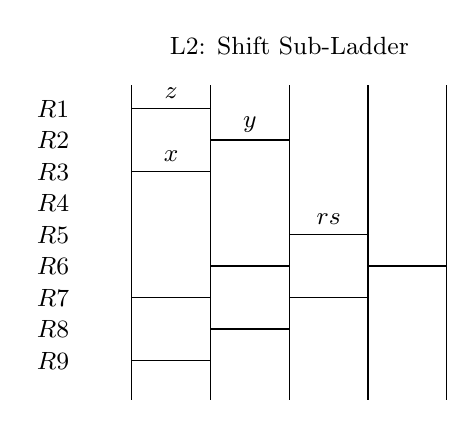
\begin{tikzpicture}
			\node at(2, 3.5){\small{L2: Shift Sub-Ladder}};

			\draw(0, -1) to (0, 3);
					\node at(.5, 2.9){\small{$z$}};
				\draw(0, 2.7) to (1,2.7);
					\node at(.5, 2.1){\small{$x$}};

				\draw(0,1.9) to (1,1.9);
				\draw(0,.3) to (1,.3);
				\draw(0,-0.5) to (1,-0.5);
			\draw(1, -1) to (1, 3);
				\node at(1.5,2.5){\small{$y$}};
				\draw(1,2.3) to (2,2.3);
				\draw(1,0.7) to (2,0.7);
				\draw(1,-0.1) to (2,-0.1);
			\draw(2, -1) to (2, 3);
				\node at(2.5, 1.3){\small{$rs$}};
				\draw(2,1.1) to (3,1.1);
				\draw(2,.3) to (3,.3);
			\draw(3, -1) to (3, 3);
				\draw(3,.7) to (4,.7);
			\draw(4, -1) to (4, 3);

			\node at(-1, 2.7){\small{$R1$}};
			\node at(-1, 2.3){\small{$R2$}};
			\node at(-1, 1.9){\small{$R3$}};
			\node at(-1, 1.5){\small{$R4$}};
			\node at(-1, 1.1){\small{$R5$}};
			\node at(-1, .7){\small{$R6$}};
			\node at(-1, .3){\small{$R7$}};
			\node at(-1, -.1){\small{$R8$}};
			\node at(-1, -.5){\small{$R9$}};


			
		\end{tikzpicture}
	\end{minipage}
		\begin{minipage}{.4\textwidth}
		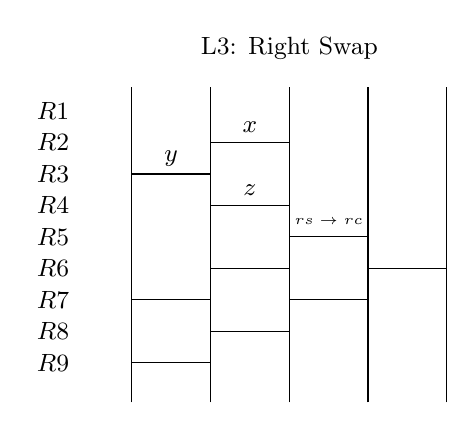
\begin{tikzpicture}
			\node at(2, 3.5){\small{L3: Right Swap}};

			\draw(0, -1) to (0, 3);
					\node at(1.5, 1.7){\small{$z$}};
				
					\node at(.5, 2.1){\small{$y$}};

				\draw(0,1.9) to (1,1.9);
				\draw(0,.3) to (1,.3);
				\draw(0,-0.5) to (1,-0.5);
			\draw(1, -1) to (1, 3);
				\node at(1.5,2.5){\small{$x$}};
				\draw(1,2.3) to (2,2.3);
				\draw(1, 1.5) to (2,1.5);
				\draw(1,0.7) to (2,0.7);
				\draw(1,-0.1) to (2,-0.1);
			\draw(2, -1) to (2, 3);
				\node at(2.5, 1.3){\tiny{$rs \rightarrow rc$}};
				\draw(2,1.1) to (3,1.1);
				\draw(2,.3) to (3,.3);
			\draw(3, -1) to (3, 3);
				\draw(3,.7) to (4,.7);
			\draw(4, -1) to (4, 3);

			\node at(-1, 2.7){\small{$R1$}};
			\node at(-1, 2.3){\small{$R2$}};
			\node at(-1, 1.9){\small{$R3$}};
			\node at(-1, 1.5){\small{$R4$}};
			\node at(-1, 1.1){\small{$R5$}};
			\node at(-1, .7){\small{$R6$}};
			\node at(-1, .3){\small{$R7$}};
			\node at(-1, -.1){\small{$R8$}};
			\node at(-1, -.5){\small{$R9$}};


			
		\end{tikzpicture}
	\end{minipage}
	\caption{$x,y,z$ to be right swapped. $rs$ is the right sibling; the root bar of the right sub-ladder.
	Going right to left, top to bottom. L1=original ladder, L2=shifting the right sub-ladder down two rows. L3 = right swap on $x,y,z$}
	\label{Fig:SwapAndShift}
\end{figure}

When a right swap operation is about to occur, bar $z$ will be moved from its current row and column to its current row + $3$ 
and its current column $+1$. Once the right swap opeartion is performed, 
the right sibling/$rs$ of $x$ becomes the right child/$rc$ of $z$.
The left swap operation is simply the inverse function of the right swap operation. 
Therefore, one can derive the left swap operation and the shift required for left swapping by deriving them 
from the right swap operation and the shift required for the right swap operation.

\begin{lemma}
	Shifting the entire sub-tree beginning at $rs$ down 
two rows ensures that $rs$ becomes $rc(z)$ and the ladder maintains its structure.
\end{lemma}
\begin{proof}
	Assume $ladder$ is a $1$ indexed two dimensional array. Going down the ladder is moving in the positive 
	direction and going up the ladder is moving in a negative direction. 
	Let $k$ be the current row of $z$. Let $k'=k+3$ be the target row of $z$. Let $m$ be the row of $rs$.
	We know that $m$ also equals the row of $x$ seeing as $rs$ is on the same row as $x$ prior to the 
	right swap operation. We know that $k$ = $m-2$ seeing as $z$ is two rows above $x$. Thus, 
	$k'=k+3=(m-2)+3=(m+1)$. Thus, the target row of $z=m+1$. Let $o$ be the current column of $z$.
	Let $o+1$ be the target column of $z$. We know that $o$ is 
	also the column of $x$ seeing as $z$ and $x$ are in the same column. 
	Thus, we know that the column of $rs$ is $o+2$ seeing as $rs$ is the right sibling  
	of $x$. Therefore the target destination of $z$ is $ladder[k'=m+1][o+1]$. 
	$rs$ is in the column $o+2$ and is at $row=m$ prior to the right swap opeartion. 
	We know that $rs \rightarrow rc(z)$ after the right swap operation, therefore $rs$ 
	must appear in the ladder at row $k'+1=m+1+1$ and the column of $o'+1$; please refer to theorem \ref{Theorem:One}
	for the definition of the right child. Since the column of $rs=o'+1$, then the column does not have to be changed.
	Since the current row of $rs$ is $m$, then the right sub-ladder needs to be shfited down by $+2$ to ensure 
	that $rs \rightarrow rc(z)$ after the right swap operation is performed. Since $rs$ also has right and left children, 
	each of them need to be shifted down two rows to ensure the ladder mainatins its structure whence the right swap 
	operation is performed. QED. 

\end{proof}


\pagebreak

%%input revoiew of second paper


\section{Ladder Lottery Realization}

In \emph{Ladder Lottery Realization}~\cite{A3}, written by Horiyama, Uno, Wasa and Yamanaka, the authors provide 
a rather interesting puzzle in regards to ladder lotteries. The puzzle 
is known as the Ladder Lottery Realization Problem. In order to understand
the problem, one must know what a \emph{multi-set} is. A \emph{multi-set}
is a set in which an element may appear more than once. The exponent 
above the element indicates the number of times it appears in the set.
For example, given the following multi-set, $\{3^{2}, 2^{4}, 5^{1}\}$ 
the element $3$ appears twice in the set, the element $2$ appears four times
in the set and the element $5$ appears once in the set.
The Ladder Lottery Realization puzzle asks, given an arbitrary starting permutation, $\pi$, 
and a multi-set of bars, 
is there a ladder lottery for $\pi$
that uses every bar in the multi-set the number 
of times it appears in the  multi-set. 
For an example of an affirmative solution to the Ladder Lottery Realization problem, see Figure~\ref{fig:ladder realization}.

\begin{figure}[!htp]
    \begin{center}
        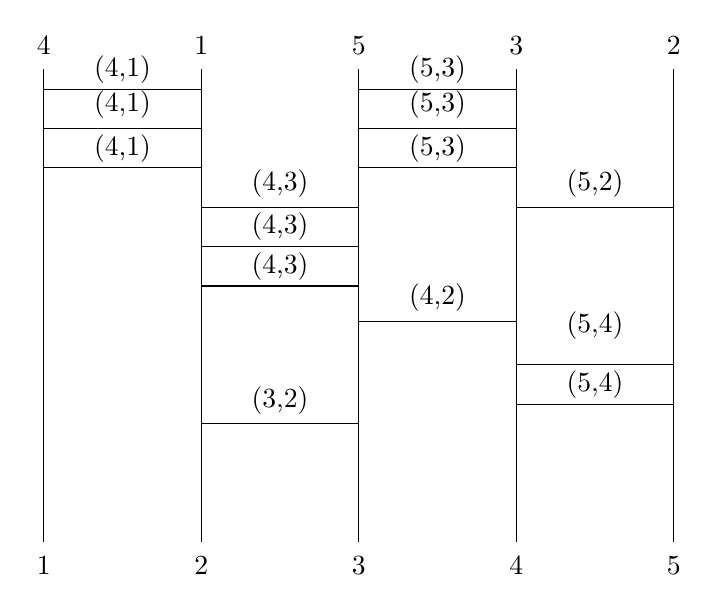
\begin{tikzpicture}
            \draw (0, 0) to (0, 6);
                \node at(0, -0.3){1};
                \node at(0, 6.3){4};
            \draw(2, 0) to (2, 6);
                \node at(2, -0.3){2};
                \node at(2, 6.3){1};
            \draw(4, 0) to (4, 6);
                \node at(4, 6.3){5};
                \node at(4, -0.3){3};
            \draw(6, 0) to (6, 6);
                \node at(6, 6.3){3};
                \node at(6, -0.3){4};
            \draw(8, 0) to (8, 6);
                \node at(8, 6.3){2};
                \node at(8, -0.3){5};

            %%draw the bars
                \node at(1, 6){(4,1)};
                    \draw(0, 5.75) to (2, 5.75);
            \draw(0, 5.25) to (2, 5.25);
                \node at(1, 5.55){(4,1)};
            \draw(0, 4.75) to (2, 4.75);
                \node at(1, 5){(4,1)};

            \draw(4, 5.75) to (6, 5.75);
                \node at(5, 6){(5,3)};
            \draw(4, 5.25) to (6, 5.25);
                \node at(5, 5.55){(5,3)};
            \draw(4, 4.75) to (6, 4.75);
                \node at(5, 5){(5,3)};

            \draw(2, 4.25) to (4, 4.25);
                \node at (3, 4.55){(4,3)};
            \draw(2, 3.75) to (4, 3.75);
                \node at (3, 4){(4,3)};
            \draw(2, 3.25) to (4, 3.25);
                \node at (3, 3.5){(4,3)};
            
            \draw(2, 1.5) to (4, 1.5);
                \node at(3, 1.8){(3,2)};
            
            \draw(4, 2.8) to (6, 2.8);
                \node at (5, 3.1){(4,2)};
            \draw(6, 4.25) to (8, 4.25);
                \node at (7, 4.55){(5,2)};
            
            \draw(6, 2.25) to (8, 2.25);
                \node at (7,2.75){(5,4)};
            
            \draw(6, 1.75) to (8, 1.75);
                \node at (7, 2){(5,4)};
            
        \end{tikzpicture}
    \end{center}
      


    \caption{An affirmative solution to the Ladder Lottery Realization Problem given a starting permutation $(4,1,5,3,2)$ and the multi set of bars $\{(3,2)^{1},(4,1)^{3}, (4,2)^{1},(4,3)^{3},(5,2)^{1},(5,3)^{3},(5,4)^{2}\}$}
    \label{fig:ladder realization}
\end{figure}
\pagebreak
The authors prove that the Ladder Lottery Realization problem in NP-Hard
by reducing the Ladder Lottery Realization to the One-In-Three 3SAT problem, 
which has already been proven to be NP-Hard.
The authors note that there are two cases in which the ladder lottery
realization problem can be solved in polynomial time. These cases 
include the following. First, if every bar in the multi-set appears
exactly once and every bar corresponds to an inversion, 
then an affirmative solution to the Ladder Lottery Realization 
instance can be achieved in polynomial time. 
Second, if there is an inversion in the permutation and its bar appears in the multi-set an even 
number of times, then a negative solution to
the Ladder Lottery Realization instance
can be achieved in polynomial time. This is because the elements that cross the bar will 
be uninverted when then be inverted again. Therefore $\pi$ will not be sorted by the ladder.\par

%%input review of third paper

\section{Optimal Reconfiguration of Optimal Ladder Lotteries}
In Optimal Reconfiguration of Optimal Ladder Lotteries, written by Horiyama, Wasa and Yamanaka,
the authors provide a polynomial solution to the 
\emph{minimal reconfiguration problem} which states that given 
two ladder is $OptL\{\pi\}$, $L_{i}$ and  $L_{m}$, what is the minimal number of 
swap operations to perform that will transition from $L_{i}$ to $L_{m}$~\cite{A2}?
The authors answer the question based on the local swap operations previously 
explained along with some other concepts. The first of these concepts 
is termed the \emph{reverse triple}~\cite{A2}. Basically, a reverse triple is a relation
between three bars, $x,y,z$ in two arbitrary ladders, $L_{i}, L_{m}$, such that if $x,y,x$
are right swapped in $L_{i}$, then they are left swapped in $L_{m}$ or if they are 
left swapped in $L_{i}$ then they are right swapped in $L_{m}$~\cite{A2}. 
The second of the concepts is the \emph{improving triple}~\cite{A2}. The improving triple is 
performing a right/left swapping three bars, $x,y,z$, in $L_{i}$ such that the 
result of the swap removes a reverse triple between
ladders $L_{i}$ and $L_{m}$~\cite{A2}. The improving triple is a symmetric 
relation, therefore performing a right/left swapping of the $x,y,z$ in $L_{m}$ also results in the 
removal of a reverse triple between $L_{i}$ and $L_{m}$~\cite{A2}.\par
The \emph{minimal length reconfiguration sequence} is the minimal number of 
improving triples required to transition from $L_{i}$ to $L_{m}$ or 
$L_{m}$ to $L_{i}$~\cite{A2}. Transitioning from $L_{i}$ to $L_{m}$ with the minimal length reconfiguration sequence 
is achieved by applying an improving triple to each of the reverse triples between 
$L_{i}$ and $L_{m}$. That is to say, the length of the reconfiguration sequence 
is equal to the number of improving triples required to remove all reverse triples between $L_{i}$ and  $L_{m}$~\cite{A2}.\par
The second contribution of this paper is that it provides a closed form formula for the 
upper bound for the minimal length reconfiguration sequence for any permutation 
of size $n$~\cite{A2}. That is to say, given some arbitrary $\pi$ of order $n$, what is the maximum 
length of the minimal length reconfiguration sequence between two ladders in $OptL\{\pi\}$?
The authors prove that there are two unique ladders in $OptL\{\pi=(n, n-1, \dots, 1)\}$ that 
have the upper bound for the minimal length reconfiguration sequence~\cite{A2}. These ladders are the root ladder and \emph{terminating ladder} in 
$OptL\{\pi=(n, n-1, \dots, 1)\}$ that have a minimal reconfiguration sequence equal to 
the upper bound. The terminating ladder in $OptL\{\pi=(n, n-1, \dots, 1)\}$ is defined as the ladder 
such that every possible right swap operation has been performed. The length of the reconfiguration sequence 
between the root ladder and terminating ladder in $OptL\{\pi=(n, n-1, \dots, 1)\}$ is $n{(n-1)~\choose 2}$~\cite{A2}. 
This is because the number of reverse triples between the root ladder and the terminating ladder 
in $OptL\{\pi(n, n-1, \dots, 1)\}$ is equal to $n{(n-1)~\choose 2}$. Thus, in 
order to reconfigure the root to the terminating ladder, or vice versa, each 
reverse triple between them must be improved by applying one improving triple.
\par

%%input review of fourth paper.

\section{Efficient Enumeration of all Ladder Lotteries with K Bars}

In this paper, the authors apply the same algorithm used in Efficient Enumeration of Optimal Ladder-Lotteries 
and its Application for generating all ladder lotteries with k bars. The number of elements 
in The inversion set of $\pi$ also known as $Inv\{\pi\}$ provides the lower bound for $K$ 
and the upper bound is positive infinity. Therefore $K=[|Inv\{\pi\}| \dots N]$\par\par 
\subsection{Coding Latter Lotteries}
\subsubsection{Overview}
In this paper, the authors provide three methods to encode ladder-lotteries as 
binary strings. Coding discrete objects as binary strings is an appealing theme because 
it allows for compact represntation of them for a computer \cite{A5}.
\subsubsection{Route Based Encoding}
The first method is termed \emph{route based encoding method} in 
which each route of an element in the permutation has a binary encoding. Let $L$
be a ladder-lottery for some arbitrary permutation $\pi$ of order $N$. The route 
of element $p_{i}$ is encoded by keeping in mind $p_{i}$ crosses bars in its route 
going left zero or more times and crosses bars in its route going right zero or 
more times \cite{A5}. The maximum number of bars $p_{i}$ can have is $N-1$, therefore the 
upper bound for the number of left/right crossings for $p_{i}$ is $N-1$ \cite{A5}. 
Let a left crossing be denoted with a $'0'$ and let a right crossing be denoted 
with a $'1'$. Let $C_{p_{i}}$ be the route encoding for the $i^{th}$ element 
in $\pi$. To construct $C_{p_{i}}$,  append $0$ and $1$ to each other representing 
the left and right crossings of $p_{i}$ from the top left 
to bottom right of the ladder \cite{A5}. If the number of crossings for $p_{i}$ 
is less than $n-1$, append $0s$ to the encoding of the route of $p_{i}$ until
the encoding is of length $N-1$ \cite{A5}. Let $LC_{L}$ be the route encoding for 
some arbitrary ladder in $OptL\{\pi\}$. $LC_{L}$ is $C_{p_{1}}, C_{p_{2}, \dots C_{p_{N}}}$.
For an example of the route encoding for the root ladder of $(3,2,5,4,1)$ refer to 
Fig.\ref{fig:route-encoding}. In \ref{fig:route-encoding}you will see that $C_{p_{1}}$ is 11\underline{00}. Underlined 
$0s$ are the $0s$ added to ensure the length of $C_{p_{1}}$ is $N-1$.
Since the length of $C_{pi}$ is $N-1$ and the number of elements in $\pi$ is $N$
then the length of $LC_{L}=N(N-1)$. Hence the number of bits needed for $LC_{L}$ 
belongs to $\mathcal{O}(N^{2})$.\par 
\begin{figure}[!htp]
    \begin{center}
        \begin{tikzpicture}
    
            %%draw the lines
            \draw(0, 0) to (0, 4);
                \node at(0, 4.3){3};
                \node at(0, -0.3){1};
            \draw(2, 0) to (2, 4);
                \node at (2, 4.3){2};
                \node at(2, -0.3){2};
            \draw(4, 0) to (4, 4);
                \node at (4, 4.3){5};
                \node at (4, -0.3){3};
            \draw(6, 0) to (6, 4);
                \node at (6, 4.3){4};
                \node at (6, -0.3){4};
            \draw(8, 0) to (8, 4);
                \node at (8, 4.3){1};
                \node at (8, -0.3){5};
    
            %%Draw the bars
            \draw(0, 2) to (2, 2);
            \draw(2, 1.5) to (4,1.5);
            \draw(0, 1) to (2, 1);

            \draw(4, 3) to (6, 3);
            \draw(6, 2.5) to (8, 2.5);
            \draw(4, 2) to (6, 2);
        \end{tikzpicture}
    \end{center}
   
 \caption{The route encoding for the following ladder lottery is 11\underline{00}01\underline{00}11\underline{00}01\underline{00}0000}
 \label{fig:route-encoding}

\end{figure}

\subsubsection{Line Based Encoding}
The second method is termed \emph{line based encoding} which focuses 
on encoding the lines of the ladder-lottery. Each line is represented 
as a sequence of endpoints of bars. Let $L$ be an optimal ladder-lottery 
with $N$ lines and $B$ bars, then for some arbitrary line, $i$, there 
are zero or more right/left endpoints of bars that 
come into contact with $i$ \cite{A5}. Let $LC_{i}$ denote the line based encoding for line $i$.
Let $1$ denote a left end point that 
comes into contact with line $i$ and let $0$ denote a right 
end point that comes into contact with line $i$. Finally, append a $0$
to line $i$ to denote the end of the line. Then line $i$ can be 
encoded, from top to bottom, as a sequence of $1s$ and $0s$ that 
terminates in a $0$.  Given the ladder in Fig. \ref{fig:line-encoding}, 
$LC_{3}$ is $001\underline{0}$. The \underline{0} denotes 
the end of the line. Let $LC_{L}$ be the line encoding for 
some arbitrary ladder, then $LC_{L}=LC_{1}, LC_{2}, \dots LC_{N}$.
Let $L_{(4,2,3,1)}$ refer to the ladder in Fig. \ref{fig:line-encoding}, then 
$LC_{L_{(4,2,3,1)}}=11\underline{0}010\underline{0}110\underline{0}010\underline{0}0\underline{0}$\par 
In order to reconstruct $L$ from its $LC_{L}$, or in other words decode
$LC_{L}$ it is important to recognize that the first line only has left endpoints attached to it
\cite{A5}. Since left end points are encoded as a $1$ then it is guarenteed that the first $0$ 
represents the end of line $1$. Secondly, the last/$Nth$ line 
has only right end points attached to it.  Therefore $LC_{N}$ will only have $0s$. Therefore, $LC_{N}$
does not require a terminating $0$. Thirdly, for any 
line $i+1$, if line $i+1$ has a $0$ then there must be a corresponding $1$
in line $i$. That is to say, if the right end point of a bar is on line 
$i+1$ then that same bar must have a left endpoint on line $i$. To decode 
$LC_{L}$ start by decoding line $1$. The line will contain $0$ or more 
left end points. To decode $LC_{i+1}$ where $i+1>1$, go to 
$LC_{i}$ and match each $1$ in $LC_{i}$ with a $0$ in $LC_{i+1}$. 
Let $k=$ the number of $1s$ in $LC_{i}$. Let $j=$ the number 
of $0s$ in $LC_{i+1}$ then $k=j-1$; due to the last $0$ in $LC_{i+1}$ denoting 
the end of line $i+1$.  Intuitively, this means match every left end point 
of a bar in line $i$ with a right end point in line $i+1$. The last $0$
represents the end of line $i+1$. For an example of a full decoding of $LC_{L_{(4,2,3,1)}}$
please refer to Fig. \ref{fig:line-encoding}.\pagebreak
\begin{figure}[!htp]
    \begin{center}
        \begin{tikzpicture}
            \draw(0, 0) to (0, 4);
            \node at (0, 4.3){4};
            \node at (0, -0.3){1};
        \draw(2, 0) to (2, 4);
            \node at (2, 4.3){2};
            \node at (2, -0.3){2};
        \draw(4, 0) to (4, 4);
            \node at (4, 4.3){3};
            \node at (4, -0.3){3};
        \draw(6, 0) to (6, 4);
            \node at (6, 4.3){1};
            \node at (6, -0.3){4};

        %%bars 
        \draw(0, 3) to (0.7, 3);
            \node at (0.35, 3.3){1};
        \draw (1.3, 3) to (2, 3);
            \node at (1.65, 3.3){0};

        \draw(2, 2.5) to (2.7, 2.5);
            \node at (2.35, 2.8){1};
        \draw(3.3, 2.5) to (4, 2.5);
            \node at (3.65, 2.8){0};

        \draw(4, 2) to (4.7, 2);
            \node at (4.35, 2.3){1};
        \draw(5.3, 2) to (6, 2);
            \node at (5.65, 2.3){0};

      

        \draw(2, 1) to (2.7, 1);
            \node at (2.35, 1.3){1};
        \draw(3.3, 1) to (4, 1);
            \node at (3.65, 1.3){0};

        \draw(0, 0.5) to (0.7, 0.5);
            \node at (0.35, 0.8){1};
        \draw(1.3, 0.5) to (2, 0.5);
            \node at (1.65, 0.8){0};

        \end{tikzpicture}
      

    \end{center}
    \caption{$LC_{L(4,2,3,1)}=LC_{1}=11\underline{0},LC_{2}=0110\underline{0},LC_{3}=010\underline{0},LC_{4}=0$}
    \label{fig:line-encoding}
\end{figure}

Since each bar is encoded as two bits, and there are $N-1$ bits as terminating bits; 
one for each line in $L$, then the number of bits required is $N + 2B -1$, where $N$
is the number of lines and $B$ is the number of bars. Encoding and decoding can be 
done in $\mathcal{O}(n+b)$ time.\cite{A5} Clearly the line-based encoding 
trumps the route-based encoding in both time and space complexity.

\subsubsection{Improved Line-Based Encoding}
Although the line-based encoding is better than the route based 
encoding, it can still be further optimized. The authors provide 
three improvements to the line-based encoding. These three improvements
can be combined to really help imrpove the line based encoding's 
space efficiency \cite{A5}. 
\paragraph{Imrpovement 1}
Since the $Nth$ line has only right endpoints attached to it, 
then it actually does not need to be encoded. Right endpoints 
are denoted as $0$ and left endpoints are encoded as $1$, therefore the number of right endpoints 
for line $N$ is equal to the number of $1s$ in $LC_{N-1}$.
Thus, there is no need for $LC_{N}$ \cite{A5}. The encoding with improvment 
one for the ladder in Fig. \ref{fig:line-encoding} is $11\underline{0}0110\underline{0}010$.
\paragraph{Improvement 2}
Improvement two is based off of the fact that for any two bars,
$x,y$, let $l_{x}$ denote the left endpoint of bar $x$, let 
$l_{y}$ denote the left endoint of bar $y$, let $r_{x}$ denote 
the right end point of bar $x$ and let $r_{y}$ denote the right 
end point of bar $y$. Let line $i$ be the line of $l_{x}$ and $l_{y}$
and let line $i+1$ be the line of $r_{x}$ and $r_{y}$.
\begin{lemma}
There are three possible cases for the 
placement of $x$ and $y$ in some 
arbitrary ladder from $OptL\{\pi\}$. The first case is that there 
is at least one other bar, $z$, with a right end point, $r_{z}$ between $l_{x}$
and $l_{y}$ on line $i$. The second case is that there is at least one other bar 
$z$, with a left end point, $l_{z}$, between $r_{x}$ and $r_{y}$ on line $i+1$. 
The third case is that there is at least one bar, $z$, with a right end point, 
$r_{z}$, betwen $l_{x}$ and $l_{y}$ on line $i$ and there is at least one other bar, 
$z\prime$ with a left end point, $l_{z\prime}$, between $r_{x}$ and $r_{y}$ on line $i+1$ \cite{A5}. 
For an example of all three cases refer to Fig. \ref{fig:three-cases}\par
\end{lemma}

%%figure demonstrating the three cases for bar positions
\begin{figure}[!htp]
       
            %%first case
            \begin{minipage}{.3\textwidth}
                \begin{tikzpicture}
                    \draw(0, 0) to (0, 4);
                        \node at (2, 4.3){\small{$i+1$}};
                    \draw(1, 0) to (1, 4);
                        \node at (1, 4.3){\small{$i$}};
                    \draw(2, 0) to (2, 4);
                        \node at (0, 4.3){\small{$i-1$}};
                    \draw(0, 2) to (1, 2);
                        \node at (.5, 2.3){\small{$r_{z}$}};
                    \draw(1, 3) to (2, 3);
                        \node at (1.5, 3.3){\small{$l_{x}$}};
                    \draw(1, 1) to (2, 1);
                        \node at (1.5, 1.3){\small{$l_{y}$}};
                \end{tikzpicture}
            \end{minipage}
              \begin{minipage}{.3\textwidth}

                 \begin{tikzpicture}
                
                  \draw(0, 0) to (0, 4);
                     \node at (0, 4.3){\small{$i-1$}};
                  \draw(1, 0) to (1, 4);
                    \node at (1, 4.3){\small{$i$}};
                  \draw(2, 0) to (2, 4);
                     \node at (2, 4.3){\small{$i+1$}};
                   \draw(0, 3) to (1, 3);
                         \node at (.5, 3.3){\small{$r_{x}$}};
                    \draw(1, 2) to (2, 2);
                         \node at (1.5, 2.3){\small{$l_{z}$}};
                     \draw(0, 1) to (1, 1);
                         \node at (0.5, 1.3){\small{$r_{y}$}};
                
                   
                
                \end{tikzpicture}
             \end{minipage}
             \begin{minipage}{.3\textwidth}

                \begin{tikzpicture}
                
                 \draw(0, 0) to (0, 4);
                    \node at (1, 4.3){\small{$i$}};
                 \draw(1, 0) to (1, 4);
                    \node at (2, 4.3){\small{$i+1$}};
                 \draw(2, 0) to (2, 4);
                    \node at (0, 4.3){\small{$i-1$}};
                 \draw(3, 0) to (3, 4);
                    \node at (3, 4.3){\small{$i+2$}};
                    \draw(1, 3) to (2, 3);
                        \node at (1.3, 3.3){\small{$l_{x}$}};
                        \node at (1.7, 3.3){\small{$r_{x}$}};
                     \draw(0, 2) to (1, 2);
                        \node at (0.7, 2.3){\small{$r_{z}$}};
                    \draw(1, 1) to (2, 1);
                        \node at (1.3, 1.3){\small{$l_{y}$}};
                         \node at (1.7, 1.3){\small{$r_{y}$}};
                     \draw(2, 2) to (3, 2);
                        \node at (2.3, 2.3){\small{$l_{z\prime}$}};
                
                   
                
                \end{tikzpicture}
            \end{minipage}
        

    \caption{Three examples of the three cases for the placement 
    of bars $x$ and $y$ in a ladder-lottery}
    \label{fig:three-cases}
\end{figure}
\begin{proof}
    Suppose that none of the above cases hold. Let $L_{\pi}$ be an 
    optimal ladder-lottery with bars $x$ and 
    bar $y$. If none of the cases hold then $x$ and $y$ are directly above/below each other without 
    the enpoint of some third bar $z$ between $l_{x}$ and $l_{y}$ or between $r_{x}$ and $r_{y}$.
    Let $x$ be the bar for the inversion of two elements $p$ and $q$ in $\pi$. 
    As $p$ and $q$ travel through the ladder they will cross each other at bar $x$; 
    thus uninverting them. Since bar $y$ is directly below bar $x$, then $p$ and $q$ will cross 
    bar $y$ thus re-inverting them. Therefore, there will need to be a third 
    bar that uninverts $p$ and $q$ a second time. Since this third bar is 
    redundant, $L_{\pi}$ is non-optimal which is a contradiction. Let $x$ be a bar for two 
    elements in $\pi$, $p$ and $q$ such that $p$ and $q$ do not form an inversion. Then $x$ 
    will invert $p$ and $q$ and $y$ will uninvert them. Thus making both $x$ and $y$ redundant
    bars which is also a contradiction. Therefore one of the above cases must hold.
\end{proof}
Knowing that one of the three above cases must hold is beneficial for improving the 
line-based encoding. If $l_{x}$ and $l_{y}$ on line $i$ have no $r_{z}$ between them, 
then there must be at least one $l_{z\prime}$ between $r_{x}$ and $r_{y}$ on line $i+1$.
Since a left endpoint is encoded as a $1$ and a right endpoint is encoded as a $0$, 
a $1$ can be omitted for the encoding of line $i+1$ if $l_{x}$ and $l_{y}$ have no $r_{z}$
between them on line $i$ \cite{A5}. That is to say, if there is not a $0$ between 
the two  $1s$ for $l_{x}$, $l_{y}$ in $LC_{i}$, it is implied that there is at least one $1$ between 
the two $0s$ for $r_{x}$, $r_{y}$ on $LC_{i+1}$. Hence, one of the $1s$ in $LC_{i+1}$ can be omitted. 
The line encoding with improvement two for the ladder in Fig. \ref{fig:line-encoding} is $11\underline{0}010\underline{0}00\underline{0}0$.
\paragraph{Imrpovement 3}
Improvement three is based off of saving some bits for right 
end points/$0s$ in $LC_{N-1}$. Since line $N$ has no left end points,
then then there must be some right endpoints between any two 
consecutive bars connecting lines $N-1$ and line $N$. If you 
refer to Fig. \ref{fig:improvement3}, then the only configuration for lines $N-2, N-1, N$
is the middle configuration \cite{A5}. Knowing this, then 
given two bars, $x$ and $y$ with $l_{x}$/$l_{y}$ on line 
$n-1$ and $r_{x}$/$r_{y}$ on line $n$, there must be at least 
one bar, $z$, with its $r_{z}$ between $l_{x}$ and $l_{y}$
on line $N-1$. Thus, for every $1$ in $LC_{N-1}$ except the 
last $1$ in $LC_{N-1}$, a $0$ must immidediately proceed any $1$
in $LC_{N-1}$. Since this $0$ is implied, it can be removed from $LC_{N-1}$ \cite{A5}. 
For an example of improvement three with its line encoding for $LC_{N-1}$ please refer to Fig.\ref{fig:improvement3}\pagebreak
\begin{figure}[!htp]
    \centering
    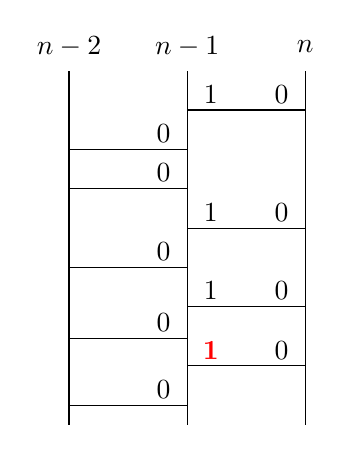
\begin{tikzpicture}
        \draw(0, -0.5) to (0, 4);
            \node at (0, 4.3){$n-2$};
            \draw(0, 3) to (1.5, 3);
                \node at (1.2, 3.2){$0$};
            \draw(0, 2.5) to (1.5, 2.5);
                \node at (1.2, 2.7){$0$};
            \draw(0, 1.5) to (1.5, 1.5);
                \node at (1.2, 1.7){$0$};
            \draw(0, 0.6) to (1.5, 0.6);
                 \node at (1.2, 0.8){$0$};
            \draw(0, -0.25) to (1.5, -0.25);
                \node at (1.2, -0.05){$0$};
        \draw(1.5, -0.5) to (1.5, 4);
            \node at (1.5, 4.3){$n-1$};
            \draw(1.5, 3.5) to (3, 3.5);
                \node at (1.8, 3.7){$1$};
                \node at (2.7, 3.7){$0$};
            \draw(1.5, 2) to (3, 2);
                \node at (1.8, 2.2){$1$};
                \node at (2.7, 2.2){$0$};
            \draw(1.5, 1) to (3, 1);
                \node at (1.8, 1.2){$1$};
                \node at (2.7, 1.2){$0$};
            \draw(1.5, 0.25) to (3, 0.25);
                \node at (1.8, 0.45){$\textcolor{red}{\textbf{1}}$};
                \node at (2.7, 0.45){$0$};

        \draw(3, -0.5) to (3, 4);
            \node at (3, 4.3){$n$};
    \end{tikzpicture}
    \caption{The line coding for $LC_{N-1}$ with imrpovement three is $101110$\underline{$0$}. The red, bold $1$ represents 
    the last left end point in $LC_{N-1}$, therefore the proceeding $0$ must be 
    included in $LC_{N-1}$. For every other $1$ in $LC_{N-1}$, a $0$ is omitted following 
    said $1$.}
    \label{fig:improvement3}
\end{figure}
\paragraph{Combining All Three}
The combination of all three improvements can be done independently. 
Let $IC_{L_{(4,2,3,1)}}$ be the \emph{improved line-based encoding} for $L_{(4,2,3,1)}$ 
by applying improvements 1-3 to $LC_{L_{(4,2,3,1)}}$. Recall that $LC_{L}$ denotes the line-based encoding for some ladder $L$.
$LC_{L_{(4,2,3,1)}}$ for the ladder in Fig. \ref{fig:line-encoding} is $11\underline{0}10101\underline{0}0010101\underline{0}000$.
By applying imrpovement one, we get $11\underline{0}101011\underline{0}0010101\underline{0}$. 
Notice how the last three $0s$ from $LC_{L}$ were removed because they represented $LC_{N}$.
By applying imrpovement two to improvememt one we get $11\underline{0}10011\underline{0}001001\underline{0}$.
Notice how the second, and eigth $1$ were removed because they are implied by 
the successive $0s$. By applying improvement three to the result of improvement 
two we get $11\underline{0}10011\underline{0}00101\underline{0}$. Notice how the last $0$ 
was removed from improvement two. This is because the $0$ is implied in $LC_{N-1}$
due to the configuration between of bars connecting lines $N-1$ and line $N$. The $IC_{L_{(4,2,3,1)}}$ for the ladder in fig. \ref{Fig:allthree} 
is $IC_{L_{(4,2,3,1)}}=11\underline{0}10011\underline{0}00101\underline{0}$.\pagebreak

\begin{figure}[!htp]
     \centering
    \begin{tikzpicture}
         \draw(0, 0) to (0, 4);
             \node at (0, 4.3){$n-3$};
             \draw(0, 3.5) to (1.5, 3.5);
             \draw(0, 2.5) to (1.5, 2.5);
         \draw(1.5, 0) to (1.5, 4);
             \node at (1.5, 4.3){$n-2$};
             \draw(1.5, 3) to (3, 3);
             \draw(1.5, 3.8) to (3, 3.8);
             \draw(1.5, 2) to (3, 2);
             \draw(1.5, 1) to (3, 1);
         \draw(3, 0) to (3, 4);
             \node at(3, 4.3){$n-1$};
             \draw(3, 2.5) to (4.5, 2.5);
             \draw(3, 1.5) to (4.5, 1.5);
             \draw(3, 0.5) to (4.5, 0.5);
         \draw(4.5, 0) to (4.5, 4);
             \node at(4.5, 4.3){$n$};
     \end{tikzpicture}
     \caption{A ladder used to illustrate all three improvements $IC_{L}$. $IC_{L}=11\underline{0}10011\underline{0}00101\underline{0}$}
     \label{Fig:allthree}
\end{figure}
\section{Enumeration, Counting, and Random Generation of Ladder Lotteries}

In this paper, the authors consider the problem of enumeration, counting and 
random generation of ladder lotteries with $N$ lines and $B$ bars \cite{A6}. 
It is important to note that the authors considered both optimal and 
non-optimal ladders for this paper. Nonetheless, the paper is still fruitful 
for its modelling of the problems and insights into ladder lotteries.
The authors use  the line-based encoding, $LC(l)$ for the representation of ladders 
that was discussed in the review of \textbf{Coding Ladder Lotteries}.

%%Section for enumeration
\subsection{Enumeration}
The authors denote a set of ladder lotteries with $N$ lines and 
$B$ bars as $S_{N,B}$. The problem is how to enumerate all the 
ladders in $S_{N,B}$ \cite{A6}. The authors use a \emph{forest structure}
to model the problem. A \emph{forest structure} is a set of trees 
such that each tree in the forest is dijoint union with every other 
tree in the forest. Consider $S_{N,B}$ to be a tree in a forest.
That is to say, a union disjoint subset of all ladders with $N$
lines and $B$ bars. Then $F_{N,B}$, or the forest of all $S_{N,B}$,
is the union of all disjoint trees of ladders with $N$ lines and $B$ bars \cite{A6}. For an example 
of a forest for $F_{3,2}$ refer to Fig. \ref{fig:forest3,2}\par %figure number.

The authors create $F_{N,B}$ by defining a removal sequennce for 
each $LC(l)$ \cite{A6}. Each ladder, $l$, in 
$F_{N,B}$ is a leaf node. By removing the second last bit of $LC(L)$ the result 
is $P(LC(l))$ and the resulting substructure is some \emph{sub-ladder}, $P(l)$, which 
is an incomplete ladder containing unmatched endpoints of bars and/or a missining line \cite{A6}. For example, 
given $LC(l)=10100$, $P(LC(l))=1010$. Notice how the second last bit was removed. 
By removing the second last bit from $P(LC(l))$ we get $P(P(LC(l)))$ and $P(P(L))$ respectively.
The removal sequence is repeated until the sub-ladder consists of two lines with $0$ endpoints
attached to line $2$ and $0$ to $r$ left endpoints are attached to line $1$. There are $r+1$
terminating sub-ladders, i.e., roots of trees in $F_{N,B}$.The removal sequence is uniqe for each ladder in $F_{N,B}$ is unique.\par
\begin{figure}[!htp]
    \begin{center}
    \begin{minipage}{.8\textwidth}
        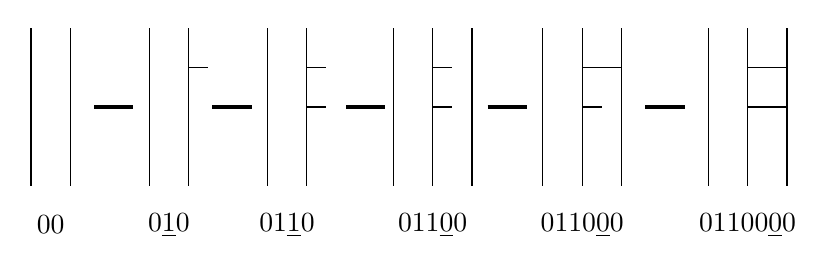
\begin{tikzpicture}
            \draw(0, 0) to (0, 2);
            \draw(0.5, 0) to (0.5, 2);
                \node at(0.25, -0.5){00};

            %%branch
            \draw[line width=0.5mm] (0.8, 1) to (1.3, 1);

            \draw(1.5, 0) to (1.5, 2);
                \draw(2, 1.5) to (2.25, 1.5);
            \draw(2, 0) to (2, 2);
                \node at (1.75, -0.5){0\underline{1}0};
    
            %%branch
            \draw[line width=0.5mm] (2.3, 1) to (2.8, 1);
            
            \draw(3, 0) to (3, 2);
            \draw(3.5, 0) to (3.5, 2);
                 \draw(3.5, 1.5) to (3.75, 1.5);
                 \draw(3.5, 1) to (3.75, 1);
                \node at (3.25, -0.5){01\underline{1}0};
            
            \draw[line width=0.5mm] (4, 1) to (4.5, 1);

            \draw(4.6, 0) to (4.6, 2);
            \draw(5.1, 0) to (5.1, 2);
            \draw(5.6, 0) to (5.6, 2);
                 \draw(5.1, 1.5) to (5.35, 1.5);
                 \draw(5.1, 1) to (5.35, 1);
                \node at (5.1, -0.5){011\underline{0}0};


            \draw[line width=0.5mm](5.8, 1) to (6.3, 1);
            \draw(6.5, 0) to (6.5, 2);
            \draw(7, 0) to (7, 2);
            \draw(7.5, 0) to (7.5, 2);
                \draw(7, 1.5) to (7.5, 1.5);
                \draw(7, 1) to (7.25, 1);
                \node at (7, -0.5){0110\underline{0}0};

            \draw[line width=0.5mm](7.8, 1) to (8.3, 1);
            \draw(8.6, 0) to (8.6, 2);
            \draw(9.1, 0) to (9.1, 2);
            \draw(9.6, 0) to (9.6, 2);
                \draw(9.1, 1.5) to (9.6, 1.5);
                \draw(9.1, 1) to (9.6, 1);
                \node at (9.1, -0.5){01100\underline{0}0};

        \end{tikzpicture}
        
    \end{minipage}
    \end{center}
    
    
  

    %%second tree
    \begin{center}
          \begin{minipage}{0.8\textwidth}
            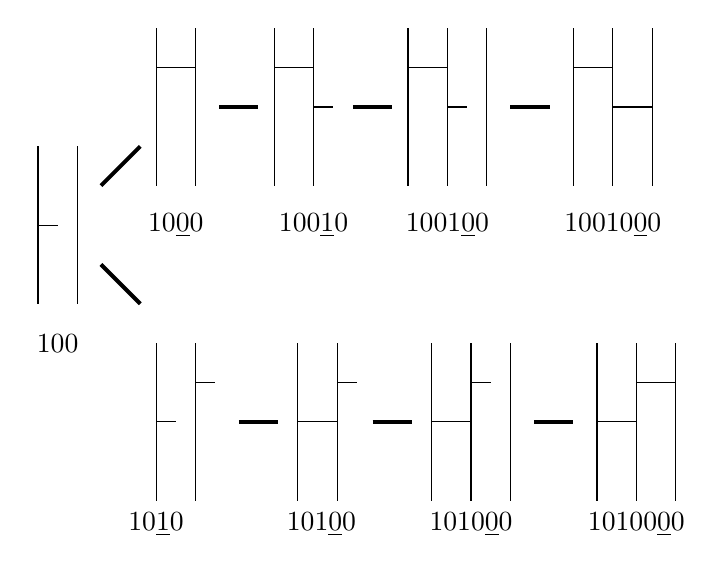
\begin{tikzpicture}
                \draw(0, 0) to (0, 2);
                \draw(0.5, 0) to (0.5, 2);
                    \draw(0, 1) to (0.25, 1);
                    \node at (0.25, -0.5){$100$};
                
                %%upper subtree
                \draw[line width=0.5mm](0.8, 1.5) to (1.3, 2);
                    \draw(1.5, 1.5) to (1.5, 3.5);
                    \draw(2, 1.5) to (2, 3.5);
                        \draw(1.5, 3) to (2, 3);
                        \node at (1.75, 1){$10\underline{0}0$};

                    \draw[line width=0.5mm](2.3, 2.5) to (2.8, 2.5);
                        \draw(3, 1.5) to (3, 3.5);
                            \draw(3, 3) to (3.5,3);
                            \draw(3.5, 2.5) to (3.75, 2.5);
                        \draw(3.5, 1.5) to (3.5, 3.5);
                        \node at (3.5, 1){$100\underline{1}0$};

                    \draw[line width=0.5mm](4, 2.5) to (4.5, 2.5);
                        \draw(4.7,  1.5) to (4.7, 3.5);
                            \draw(4.7, 3) to (5.2, 3);
                            \draw(5.2, 2.5) to (5.45, 2.5);
                        \draw(5.2, 1.5) to (5.2, 3.5);
                        \draw(5.7, 1.5) to (5.7, 3.5);
                        \node at (5.2, 1){$1001\underline{0}0$};

                    \draw[line width=0.5mm](6, 2.5) to (6.5, 2.5);
                        \draw(6.8,  1.5) to (6.8, 3.5);
                            \draw(6.8, 3) to (7.3, 3);
                            \draw(7.3, 2.5) to (7.8, 2.5);
                        \draw(7.3, 1.5) to (7.3, 3.5);
                        \draw(7.8, 1.5) to (7.8, 3.5);
                        \node at (7.3, 1){$10010\underline{0}0$};



                %%lower subtree
                \draw[line width = 0.5mm](0.8, 0.5) to (1.3, 0);
                    \draw (1.5, -0.5) to (1.5, -2.5);
                        \draw(1.5, -1.5) to (1.75, -1.5);
                        \draw(2, -1) to (2.25, -1);
                    \draw(2, -0.5) to (2, -2.5);
                        \node at (1.5, -2.8){$10\underline{1}0$};
                    
                    \draw[line width = 0.5mm](2.55, -1.5) to (3.05, -1.5);

                     \draw (3.3, -0.5) to (3.3, -2.5);
                        \draw(3.3, -1.5) to (3.8, -1.5);
                        \draw(3.8, -1) to (4.05, -1);
                    \draw(3.8, -0.5) to (3.8, -2.5);
                        \node at (3.6, -2.8){$101\underline{0}0$};

                     \draw[line width = 0.5mm](4.25, -1.5) to (4.75, -1.5);

                     \draw (5, -0.5) to (5, -2.5);
                        \draw(5.5, -1) to (5.75, -1);
                        \draw(5, -1.5) to (5.5, -1.5);
                    \draw(5.5, -0.5) to (5.5, -2.5);
                    \draw(6, -0.5) to (6, -2.5);
                        \node at (5.5, -2.8){$1010\underline{0}0$};
                    

                    \draw[line width = 0.5mm](6.3, -1.5) to (6.8, -1.5);
                    \draw (7.1, -0.5) to (7.1, -2.5);
                        \draw(7.1, -1.5) to (7.6, -1.5);
                        \draw(7.6, -1) to (8.1, -1);
                    \draw(7.6, -0.5) to (7.6, -2.5);
                    \draw(8.1, -0.5) to (8.1, -2.5);
                        \node at (7.6, -2.8){$10100\underline{0}0$};
                    

                    
            \end{tikzpicture}
            
        \end{minipage}
    \end{center}


    \begin{center}
        \begin{minipage}{0.8\textwidth}
            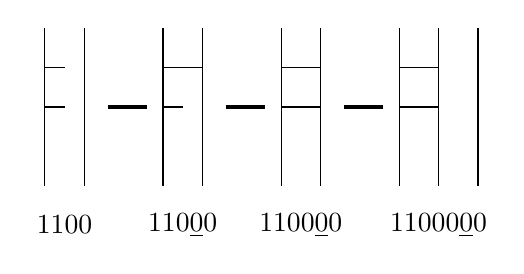
\begin{tikzpicture}%% start pocture
            
            
                \draw(0, 0) to (0, 2);
                    \draw(0, 1.5) to (0.25, 1.5);
                    \draw(0, 1) to (0.25, 1);
                \draw(0.5, 0) to (0.5, 2);
                \node at (0.25, -0.5){$1100$};
            
            
                \draw[line width=0.5mm] (0.8, 1) to (1.3, 1);
                    \draw(1.5, 0) to (1.5, 2);
                        \draw(1.5, 1.5) to (2, 1.5);
                        \draw(1.5, 1) to (1.75, 1);
                    \draw(2, 0) to (2, 2);
                    \node at (1.75, -0.5){$110\underline{0}0$};
            
        
                \draw[line width=0.5mm] (2.3, 1) to (2.8, 1);
                    \draw(3, 0) to (3, 2);
                       \draw(3, 1.5) to (3.5, 1.5);
                       \draw(3, 1) to (3.5, 1);
                   \draw(3.5, 0) to (3.5, 2);
                    \node at (3.25, -0.5){$1100\underline{0}0$};
            
            
                \draw[line width=0.5mm] (3.8, 1) to (4.3, 1);
                    \draw(4.5, 0) to (4.5, 2);
                          \draw(4.5, 1.5) to (5, 1.5);
                          \draw(4.5, 1) to (5, 1);
                      \draw(5, 0) to (5, 2);
                      \draw(5.5, 0) to (5.5, 2);
                          \node at (5, -0.5){$11000\underline{0}0$};
               
            \end{tikzpicture}%%end picture
        \end{minipage}
    \end{center}
    \caption{The forest, $F_{3,2}$ where $3$ is the number of lines and $2$ is the number of bars. All ladders with $3$ lines and $2$ bars are leaf nodes of one of three trees $S_{3,2}$.
    The underlined bits are the inserted second last bit from the parent's line-encoding resulting in the child's line encoding}
    \label{fig:forest3,2}
\end{figure}

%%end enumeratiom section

%%section for counting
\subsection{Counting}
The authors provide a method and algorithm to count all ladders 
with $N$ lines and $B$ bars. According to the authors, the enumeration algorithm is 
much slower than the counting algorithm \cite{A6}. The counting algorithm 
works by dividing ladders into four types of sub-ladders.
For sub-ladder, $r$, its type is a tuple $t(n,h,p,q)$ where 
$n$ is the number of lines, $h$ is the number of half bars, 
$p$ is the number of unmatched end-points on line $n-1$ and 
$q$ is the number of unmatched end-points on line $n$. From this 
type there are four sub-divisions of sub-ladders.\cite{A6}
\subsubsection{ $h < p+q$ or $n<2$}
There are zero ladders because it is impossible for the 
root sub-ladder to have less than two lines. It is also 
impossible for the number of half bars, $h$, to 
be less than the number of detached left end points 
on line $n-1$ plus the number of detached end points on 
line $n$.

%%\subsubsubsection{Case 2: $n=2$ and $h=p$ and $q=0$}
\subsubsection{$n=2$ and $h=p$ and $q=0$}
There is only one ladder because the number of half bars 
on the last line is 0 since $q=0$. Therefore all half bars are on the 
$n-1th$ line of the sub-ladder. This is known because 
$h=p$ which means the number of half bars is the same as 
the number of unmatched bars on line $n-1$. Hence, the unmacthed 
half bars on the $n-1th$ line must be connected to the $n$ 
line. Once these are all matched the ladder will be complete. 
Thus, there is only one ladder for this case.

%%\subsubsubsection{Case 3: $(n \geq 3$ or $h>p)$ and $q=0$}
\subsubsection{$(n \geq 3$ or $h>p)$ and $q=0$}
If this is the case, then there are no endpoints attached to 
line $n$, but the number of half bars is greater than the 
number of enpoints attached to line $n-1$, which means there is 
some line(s) $n-t$, $t>2$ that have end points attached to them.
Let $r$ be a sub-ladder of type $r=t(n,h,p,q)$
with the the above values for $n,h,p,q$. In order to count the number of ladders of type 
$t(n\geq3, h>p, q=0)$ the authors demonstrate an injection $|t(n\geq3, h>p, q=0)|=|t(n-1,h,0,p)| + |t(n,h-1,p+1,q)|$.\cite{A6}
Let $P(r)$ be $r$ with the removal of $r's$ second last bit in $LC(r)$; i.e. the parent of 
$r$.  The $LC(R)$ must have a $0$ for the second last bit. This $0$ designates either the 
end of line $n-1$ or a right endpoint of a bar attached to line $n-1$. 
If the second last bit in $LC(r)$ is the right end point of some 
bar, then $P(r)=t(n,h-1,p+1,q)$. This is because the $n-1th$ bar 
has a right end point that must be connected to some left  
endpoint at line $n-2$. Since the removal sequence of the second 
last bit ensures that there cannot be a right end-point detached 
from a left end-point. Only left end-points can be detached 
from right end-points \cite{A6}. However, if the second last bit 
of $LC(r)$ designates the end of line $n-1$, then $P(r)=t(n-1,h,0,p)$. 
This is because the removal of the second last bit 
is the removal of the end of line $n-1$ in $r$. Thus, 
line $n$ must be empty in $r$ since the last bit in $LC(r)$
designated the end of line $n$. Thus, if line $n$ is empty 
and the end point of line $n-1$ has been removed from $LC(r)$, 
resulting in $P(LC(r))$, the last bit in $P(LC(r))$ must be 
the end of line $n-1$ in $r$ resulting in a pre-ladder with one 
less line than $r$.\par  

\subsubsection{ $h\geq p+q$ and $q>0$}
%%\subsubsubsection{Case 4: $h\geq p+q$ and $q>0$}
Let $r$ be a pre-ladder of type $t(n,h,p,q)$. The authors 
demonstrate $|t(n,h\geq p+q,q>0)|=|t(n,h-1,p+1,q)|+|t(n,h-1,p,q-1)|$.\cite{A6} 
The second last bit of $LC(r)$ is either a $0$ 
or a $1$. If it is a $0$ then it represents a 
right end point attached to line $n$. Thus, 
removing it to get $P(LC(R))$ is in effect 
detaching a right end point from some left end point 
on line $n-1$. Therefore, the parent, $P(R)$ is 
of type $t(n,h-1,p+1,q)$. Seeing as in the parent, 
there is now a left end point detached from its right 
end point in $R$. However, if the second last bit 
of $LC(R)$ is a $1$, then this indicates the left 
half of a bar on line $n$. But since there is no 
bar $n+1$, this left end point must be detached. 
Therefore, by removing this $1$ in $LC(R)$ results 
in a parent with one less detached end point on line $n$.
Thus $P(R)$ is of type $t(n,h-1,p,q-1)$.
\subsection{Random Genearation}
The random generation of ladder lotteries with $N$ lines and
$B$ bars is done by the recurrence relations in the counting 
and enumerating sections. The goal is to produce 
some $L$ of type $t(n,2b,0,0)$ where the number of half 
bars equals the total $2(b)$ and there are no detached 
end points on lines $n-1$ and $n$. This implies that there 
are no detached endpoints on any line $n-t$ where $t\geq2$
because the removal sequence from the $LC(pre-ladder)$
ensures that any line before $n-1$ has no detached endpoints. Thus, 
if $L$ is of type $t(n,2b,0,0)$ it is no longer a pre-ladder 
but a complete ladder with $n$ lines and $b$ bars \cite{A6}.\par 
The authors use an algorithm to generate a random integer, $x$,
in $[1,|t(n,h,p,q)|]$. where $t(n,h,p,q)$ corresponds to some 
parent type of ladder. $t(n1,h1,p1,q1)$ corresponds to one 
child type of $t(n,h,p,q)$ and $t(n2,h2,p2,q2)$ corresponds 
to the other child type. If $x\leq|t(n1,h1,p1,q1)|$ then generate 
a pre-ladder of type $t(n1,h1,p1,q1)$ else generate a pre-ladder 
of type $t(n2,h2,p2,q2)$ \cite{A6}. Continue until there is type $t(n,2b,0,0)$
which corresponds to a complete ladder lottery with $n$ lines and $b$ bars.
\subsection{Permutations}
Ladder-lotteries and permutations are intricately related to each other. In one of the main problems addressed in this thesis, The Listing Problem, 
the research for this problem primarily came from researching listing algorithms for permutations. Four of these 
permutation listing algorithms will be presented along with their influence on the listing algorithms for The Listing Problem 
pertaining to ladder-lotteries. These four permutation listing algorithms are Heap's algorithm, Zak's algorithm, Lexicographic algorithm 
and the Steinhaus-Johnson-Trotter algorithm. 

\subsubsection{Heap's Algorithm}
Heap's algorithm was developed by B.R. Heap in 1963. The algorithm is based on rotating elements in an array such that the 
%%Sorting Networks File. 

%Intro subsection
\section{Sorting Networks}
Let a \emph{wire} be a horizontal line. Let a \emph{comparator} be a vertical line connecting two wires. A 
\emph{sorting network} is a device consisting of $[1 \dots n]$ wires and $[0 \dots m]$  
comparators such that the sorting network sorts a permutation of $n$ elements into ascending order. The 
$n$ elements are first listed to the left of each wire in the network. The elements travel across their respective wires 
at the same time. When a pair of elements, traveling through a pair of wires, 
encounter a comparator, the comparator swaps the elements if and only if the top wire's element 
is greater than the bottom wire's element. A sorting network with $n$ wires and $m$ 
comparators that can sort any permutation of order $n$ is a \emph{complete sorting network}. 
To see a complete sorting network for $n=4$ please refer to Figure~\ref{Fig:SortNetwork}.\par 

\begin{figure}[h]
   ~\centering
    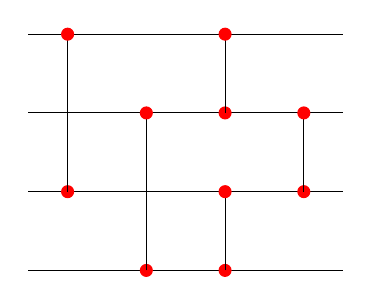
\begin{tikzpicture}
        \draw(0, 0) to (4, 0);
           
        \draw(0, 1) to (4, 1);
        \draw(0, 2) to (4, 2);
           
        \draw(0, 3) to (4, 3);

        %%connector 1
        \draw[red, fill=red](.5,1) circle (.5ex);
            \draw(.5, 1) to (.5, 3);
        \draw[red, fill=red](.5,3) circle (.5ex);


        %%connector 2 
        \draw[red, fill=red](1.5,0) circle (.5ex);
            \draw(1.5, 0) to (1.5, 2);
        \draw[red, fill=red](1.5,2) circle (.5ex);

        %%connector 3
        \draw[red, fill=red](2.5,2) circle (.5ex);
            \draw(2.5, 2) to (2.5, 3);
        \draw[red, fill=red](2.5,3) circle (.5ex);

        \draw[red, fill=red](2.5,0) circle (.5ex);
            \draw(2.5, 0) to (2.5, 1);
        \draw[red, fill=red](2.5,1) circle (.5ex);
        
        %%connector 4
        \draw[red, fill=red](3.5,1) circle (.5ex);
            \draw(3.5, 1) to (3.5, 2);
        \draw[red, fill=red](3.5,2) circle (.5ex);


    \end{tikzpicture}
    \caption{Complete Sorting Network for $n=4$.}
    \label{Fig:SortNetwork}
\end{figure}

Sorting networks were first studied in 1954 by Armstrong, Nelson and O'Connor. 
Sorting networks can be implemented either in hardware or in software~\cite{A18}.
Donald Knuth describes how the comparators for binary integers can be implemented as simple, 
three-state electronic devices~\cite{A18}. Batcher, in 1968, 
suggested using them to construct switching networks for computer hardware, replacing 
both buses and the faster, but more expensive, crossbar switches~\cite{A27}. Since the 2000s, sorting networks are used by the 
\emph{general purpose graphics processing unit community}, which are a group of people who use 
the GPU for non-graphical programming, for constructing sorting algorithms~\cite{A28}.\par 
Sorting networks are intricately related to ladder-lotteries. Let a \emph{minimum sorting network} be defined 
as a sorting network such that for any arbitrary comparator, $c$, on wire $i$, $c$ connects to line $i+1$ or $i-1$. Furthermore, 
the number of comparators in a minimum sorting network is equal to the number of inversions in $\pi$. Clearly there is a 
one to one mapping from the comparators in a minimum sorting network to the bars in an optimal ladder lottery and there 
is a one to one mapping from the wires in a minimum sorting network and the lines in a ladder lottery~\cite{A29}. 


 
\subsection{The Integer Sequence Relating to the Reverse Permutation}
Let $Rev(\pi)$ refer to the reverse permutation of $[1 \dots n]$. There is an integer sequence that counts the number of minimum sorting networks 
for $Rev(\pi$). This integer sequence also counts $OptL\{Rev(\pi)\}$. This sequence grows very quickly, therefore $n=15$ 
is  the largest value this integer sequence has been calculated for. To refer to the table for this sequence 
please refer to Table~\ref{Tab:IntSeq1}~\cite{A30}.
\begin{table}[t]
    \begin{center}

    \begin{tabular}{|p{2cm}||p{8cm}|}
        \hline
        \multicolumn{2}{|c|}{Number of minimum sorting networks/$|OptL\{Rev(\pi)\}|$}\\
        \hline
        n & Count \\ 
        \hline 
        1 & 1 \\
        \hline 
        2 & 1 \\
        \hline 
        3 & 2 \\
        \hline 
        4 & 8 \\
        \hline 
        5 & 62 \\
        \hline 
        6 & 908 \\
        \hline 
        7 & 24698 \\
        \hline 
        8 & 1232944 \\
        \hline 
        9 & 112018190 \\
        \hline 
        10 & 18410581880 \\
        \hline 
        11 & 5449192389984 \\ 
        \hline 
        12 & 2894710651370536 \\
        \hline 
        13 & 2752596959306389652 \\
        \hline 
        14 & 4675651520558571537540 \\
        \hline 
        15 & 14163808995580022218786390 \\
        \hline 
    \end{tabular}
    \end{center}
    \caption{Number of minimum sorting networks and $|OptL\{Rev(\pi)\}|$}
    \label{Tab:IntSeq1}
\end{table}\par
According to Dumitrescu and Mandal, in their paper New Lower Bounds For The Number of Pseudoline Arrangements 
published in 2018, they have devised the current best known lower bound for this sequence to be 
$bn\geq cn^{2} − O(n log n)$ for some constant $c > 0.2083$. In particular, $bn \geq 0.2083 n^{2}$
for large values of $n$~\cite{A33}. Where $bn$ is the bound for a given value $n$. In the paper, Coding 
and Counting Arrangements of Pseudolines by Felsner and Valtr, written in 2011, the authors demonstrate 
the best known upper bound for this sequence is $bn \leq 2^{0.657n^{2}}$~\cite{A32}.\par 

Seeing as there is yet to be a closed form solution for this sequence, new values of $n$ are counted by a variety of algorithms. 
In the paper, Efficient Enumeration of all Ladder Lotteries and its Application, 
the authors were the first to calculate the sequence for $n=11$ with the algorithm {\sc FindAllChildren}~\cite{A1}. 
In the paper, Counting Primitive Sorting Networks by $\mathbb{\pi}$DDs, written by Kawahara, Minato, Saitoh and Yoshinaka, the authors
 were the first to calculate for $n=13$ with a data structure they have termed $\mathbb{\pi}$DD~\cite{A29}. 
 The data structure is a digraph that holds a 
set of elementary permutations along with a number of operations that are applied to the elementary permutations~\cite{A29}.
The data structure resembles a digraph with two sink nodes; one sink node is labelled the zero sink node and the other 
is labelled the one sink node~\cite{A29}.
\pagebreak





%%%section on how ladde lotteries relate to other mathematical objects
% Despite the fact that ladder lotteries have only been stuidied in and
% of themseleves for ten years, they are closely tied to other mathematical 
% phenomena that have been studied for much longer. These mathematical phenomena  
%  include \emph{Pseudo Lines} which are an arrangement of 
% curves on a plane such that given two curves, they only intersect 
% at most once and at each intersection, only two curves intersect.See figure --reference--
% for a wiring diagrams of the pseudo line arrangement for the 
% permutation, $(5,4,3,2,1)$. The other mathematical phenomena is \emph{adjacent transpositions}
% which is a swap of two adjacent elements in a permutation. 
%%\subsection{Ladders and Adjacent Transpositions}
A ladder lottery is a way of sorting a permutation, yet it can also be thought of as 
a decomposition of a permutation into \emph{adjacent transpositions}. \cite{A1} 
An \emph{adjacent transposition} is simply a swap of two adjacent elements in a 
permutation. For example, given the permutation (1, 3, 4, 2), an adjacent 
transposition could be done on the following pairs of elements: 
(1, 3), (3, 4) or (4, 2). Each would result in a unique permutation. 
Simply put, given any arbitrary starting permutation, $\pi$, keep swapping 
adjacent inversions until the identity permutation is reached.  An optimal 
ladder lottery from $\pi's$ optimal ladder set is a minimal sequence of 
adjacent transpositions such that $\pi$ is sorted into the identity permutation; 
each ladder in the set represents a sequence of adjacent transpositions for 
sorting $\pi$ into the identity permutation. For example, given the permutation 
(4, 3, 2, 1) there exists eight ladders in this permutation's optimal ladder set. 
Two of these ladders are found in \ref{fig:ac}:

\begin{figure}[!htp]
    \label{fig:ac}
	\begin{minipage}{0.4\textwidth}
		\centering
	
		\begin{tikzpicture}
			\draw(0, 0) to (0, 4) node[above]{4};
			\draw(2, 0) to (2, 4) node[above]{3};
			\draw(4, 0) to (4, 4) node[above]{2};
			\draw(6, 0) to (6, 4) node[above]{1};
			
			\draw(0, 3.7) to (2, 3.7);
				\draw node at (1, 3.9) {(4, 3)};
			\draw(2, 3.25) to (4, 3.25);
				\draw node at (3, 3.45){(4, 2)};
			\draw(4, 2.75) to (6, 2.75);
				\draw node at (5, 3.0){(4, 1)};
			
			\draw(0, 2.75) to (2, 2.75);
				\draw node at (1, 3.0){(3, 2)};
			\draw(2, 2.25) to (4, 2.25);
				\draw node at (3, 2.5){(3, 1)};
			
			
			\draw(0, 1.75) to (2, 1.75);
				\draw node at (1, 1.95){(2, 1)};
			
			\draw node at (0, -0.5){1};
			\draw node at (2, -0.5){2};
			\draw node at (4, -0.5){3};
			\draw node at (6, -0.5){4};
			
			%%second ladder%%
			\draw(9, 0) to (9, 4) node[above]{4};
			\draw(11, 0) to (11, 4)node[above]{3};
			\draw(13, 0) to (13, 4)node[above]{2};
			\draw(15, 0) to (15, 4)node[above]{1};
			
			\draw(9, 3.7) to (11, 3.7);
				\draw node at (10, 3.9) {(4, 3)};
			\draw(11, 3.25) to (13, 3.25);
				\draw node at (12, 3.45){(4, 2)};
			\draw(13, 2.75) to (15, 2.75);
				\draw node at (14, 3.0){(4, 1)};
			
			\draw(9, 1.25) to (11, 1.25);
				\draw node at (10, 1.5){(3, 1)};
			\draw(11, 2) to (13, 2);
				\draw node at (12, 2.25){(2, 1)};
			
			\draw(11, 0.65) to (13, 0.65);
				\draw node at (12, 0.85){(3, 2)};
			 
			
			\draw node at (9, -0.5){1};
			\draw node at (11, -0.5){2};
			\draw node at (13, -0.5){3};
			\draw node at (15, -0.5){4};	
		\end{tikzpicture}
	
	\end{minipage}
	

	
		
	\caption{The left ladder is one of eight unique ladders from (4,3,2,1)'s optimal ladder set. The right ladder is another one of eight unique ladders form (4,3,2,1)'s optimal ladder set}
		
\end{figure}

From looking at the above ladders, going from top left to bottom right, the left ladder represents the sequence of adjacent transpositions (4,3), (4,2), (4,1),(3,2),(3,1),(2,1) 
whereas the right ladder represent the sequence of adjacent transpositions 
(4, 3),(4, 2),(4, 1),(2, 1),(3, 1),(3, 2). 
Notice how the length of the sequences are the same,because both lengths are equal 
to the minimal number of swaps to sort (4, 3, 2, 1) 
it is simply the order in which the adjacent transpositions occur in the sequence 
that makes the sequences different from each other. 